% -*- latex -*-
% FILE: "/home/evmik/jobs/wm/2012_spring_Analog_Electronics_252/final_exam/final_exam.tex"
% LAST MODIFICATION: "Tue, 01 May 2012 11:45:17 -0400 (evmik)"
% (C) 2009 by Eugeniy Mikhailov, <evgmik@gmail.com>
% $Id:$

\documentclass[letterpaper,addpoints,answers]{exam}
\usepackage{graphicx}
\usepackage{hyperref}

\begin{document}
%\pagestyle{headandfoot}
%\lhead{
	%\large\bfseries Physics 107\\ 
	%Midterm Exam, June 15, 2009
%}
%\chead{}
%\rhead{
	%\large\bfseries Name:\enspace\makebox[2in]{\hrulefill}\\
	%\large\bfseries Signature:\enspace\makebox[2in]{\hrulefill}
%}
%\lfoot{}
%\cfoot[]{Page \thepage}
%\rfoot{}

\begin{coverpages}
	\noindent 
  \large\bfseries Physics 252

  \vspace{2ex}
	\noindent 
  Final Exam, May  2012

  \vspace{5ex}
	\noindent 
  \large\bfseries Name:\enspace\makebox[2in]{\hrulefill}\\

  \vspace{5ex}
	\noindent 
  \large\bfseries Signature:\enspace\makebox[2in]{\hrulefill}

  \vspace{5ex}
	\noindent 
	This test is administered under the rules and regulations of the honor 
	system of the College of William \& Mary.  

  \vspace{5ex}
	\noindent 
	Show your work, circle your answers.


  \vspace{5ex}
  \combinedgradetable[v][questions]
\end{coverpages}
 
\begin{questions}

	% -*- latex -*-
% FILE: "/home/evmik/jobs/wm/2012_spring_Analog_Electronics_252/final_exam/questions/filters_multi_choice.tex"
% LAST MODIFICATION: "Mon, 30 Apr 2012 23:14:28 -0400 (evmik)"
% (C) 2011 by Eugeniy Mikhailov, <evgmik@gmail.com>
% $Id:$

\question{}
	For circuits shown below specify if it a low-pass, high-pass, band-pass
	or band-reject filter. {\bf Hint:} It may be useful to think about
	transfer function at high and low frequencies.
	\begin{parts}
		\part[2]
		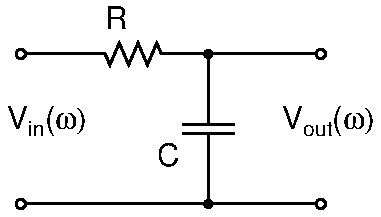
\includegraphics[height=0.7in]{./schematics/rc_low_pass}

		\part[2]
		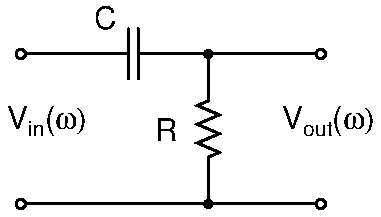
\includegraphics[height=0.7in]{./schematics/rc_high_pass}

		\part[2]
		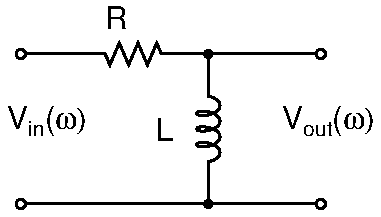
\includegraphics[height=0.7in]{./schematics/rl_high_pass}

		\part[2]
		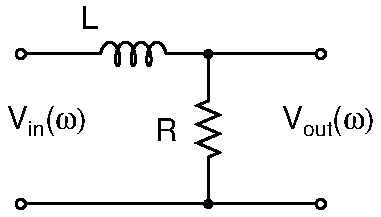
\includegraphics[height=0.7in]{./schematics/rl_low_pass}

		\part[2]
		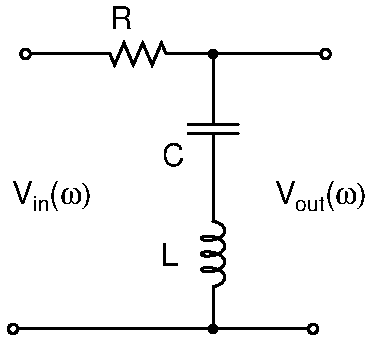
\includegraphics[height=0.7in]{./schematics/rlcnotch}

		\part[2]
		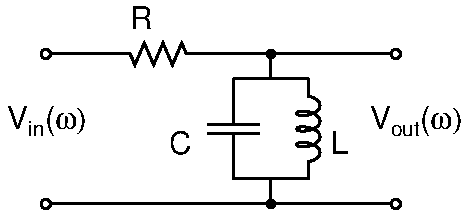
\includegraphics[height=0.7in]{./schematics/rlc_band_pass}

		\part[2]
		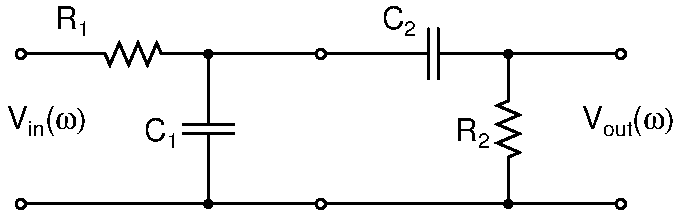
\includegraphics[height=0.7in]{./schematics/band_pass_filter}

		\part[2]
		Sketch the transfer function of the last filter (g)  in log-log
		scale.
		\vskip 1in 

		\part
		Under what conditions the last filter (g) has a transfer
		function close to unity at least in some frequency region?

		\begin{subparts}
			\subpart[2]
				Express one condition in terms of $3_{dB}$ points of the
				low-pass and high-pass filters constituting combined
				filter (g). 
			\vskip 0.5in
			\subpart[2]
				What must be true about $R_1$ and $R_2$?
		\end{subparts}


	\end{parts}
	\pagebreak


	% -*- latex -*-
% FILE: "/home/evmik/jobs/wm/2011_spring_Analog_Electronics_252/final_exam/questions/opamp_vs_transistors_comparison.tex"
% LAST MODIFICATION: "Thu, 05 May 2011 10:01:49 -0400 (evmik)"
% (C) 2011 by Eugeniy Mikhailov, <evgmik@gmail.com>
% $Id:$

\question{}
	\begin{parts}
		\part[4]
		List advantages of Op-amps when they are compared to transistors
		\vskip 3in

		\part[3]
		List situations when you would use a transistor  instead of a generic Op-amp
		\vskip 3in

		\part[3]
		What is so good about FETs when they are compared to BJTs.
		\vskip 3in
	\end{parts}
	\pagebreak


	% -*- latex -*-
% FILE: "/home/evmik/jobs/wm/2012_spring_Analog_Electronics_252/final_exam/questions/thevenin_parameters_of_a_circuit.tex"
% LAST MODIFICATION: "Mon, 30 Apr 2012 23:10:08 -0400 (evmik)"
% (C) 2011 by Eugeniy Mikhailov, <evgmik@gmail.com>
% $Id:$

\question{}
	Consider the circuit shown below \\
	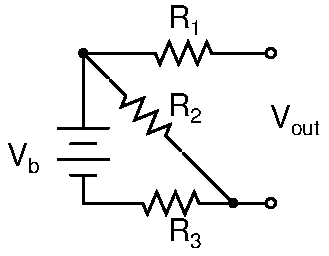
\includegraphics[width=0.25\textwidth]{./schematics/resistors_net}\\
	Where $R_1$=8~k$\Omega$, $R_2$=6~k$\Omega$, $R_3$=3~k$\Omega$, and
	the battery voltage $V_b=18$~V.\\
	{\bf Hint 1:} For solving below problems, it is helpful to mentally connect a dummy load and express {\bf
	symbolically} the $V_{out}$ vs $I_{out}$ for different $R_L$.
	{\bf Hint 2:} There is a faster way.
	\begin{parts}
		\part[8]
		What is the Th\'{e}venin voltage  of this circuit?

		\vskip 2.0in
		$V_{th}=$
		\part[8]
		What is the Th\'{e}venin resistance  of this circuit?

		\vskip 2.0in
		$R_{th}=$
		\part[5]
		If someone connected a load with resistance $R_L$=1~k$\Omega$ 
		what is the power dissipated by this load?

		\vskip 0.5in
		$P_{L}=$
		\part[4]
		While the same load connected to the circuit what is the total power
		dissipated by all resistors (excluding the load)  of the circuit
		network.


		\vskip 0.5in
		$P_{tot}=$
	\end{parts}
	\pagebreak


	% -*- latex -*-
% FILE: "/home/evmik/jobs/wm/2012_spring_Analog_Electronics_252/final_exam/questions/bjt_amplifier.tex"
% LAST MODIFICATION: "Tue, 01 May 2012 01:18:46 -0400 (evmik)"
% (C) 2011 by Eugeniy Mikhailov, <evgmik@gmail.com>
% $Id:$

\question{}
	Consider the circuit shown below \\
	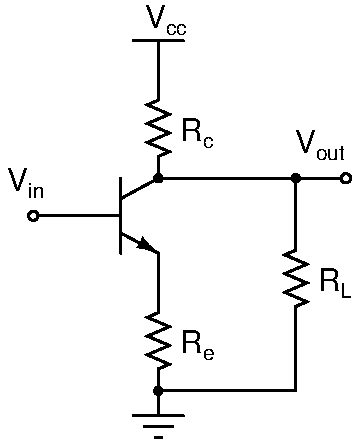
\includegraphics[height=2in]{./schematics/npn_common_emitter_amplifier}\\
	\begin{parts}
		\part[10]
		Derive the expression for the output voltage $V_{out}$, in terms of
		$V_{in}, V_{cc}, R_c, R_e,$ and  the base to emitter voltage drop $V_{be}$.
		Assume that $\beta=200$. Also assume that   the load resistor ($R_L$) is large enough and does not affect the circuit. 

		\vskip 1.5in
		$V_{out}=$
		\part[5]
		What is the small signal gain of this circuit?

		\vskip 0.5in
		$G=$
		\part[5]
		Assume that   the load resistor ($R_L$) is large enough and does not affect the circuit. 
		If $R_c/R_e=10$, $V_{be}=.6$~V and $V_{cc}=15$~V, what is
		the maximum and minimum DC
		input voltage $V_{in}$ at which this circuit  is still not saturated or railing?

		\vskip 1.0in
		$V_{{in}_{min}}=$ \hspace{2in} 
		$V_{{in}_{max}}=$
		\bonuspart[5]
		What is the output impedance of this circuit? {\bf Stating it is not
		enough, show the derivation!}

		\vskip 1.0in
		$Z_{out}=$
	\end{parts}
	\pagebreak

	% -*- latex -*-
% FILE: "/home/evmik/jobs/wm/2012_spring_Analog_Electronics_252/final_exam/questions/opamp_adder.tex"
% LAST MODIFICATION: "Mon, 30 Apr 2012 15:45:04 -0400 (evmik)"
% (C) 2011 by Eugeniy Mikhailov, <evgmik@gmail.com>
% $Id:$

\question{}
	Consider the circuit shown below \\
	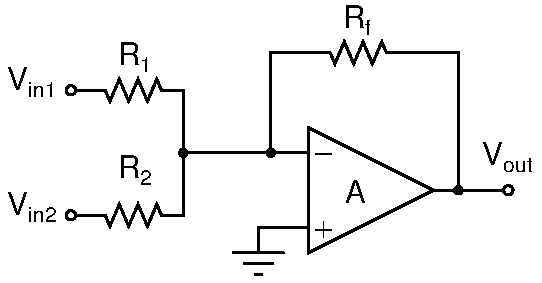
\includegraphics[height=1in]{./schematics/summing_inv_ampl}\\
	The open loop gain $A=\infty$.
	\begin{parts}
		\part[10]
		Derive the expression for the output voltage $V_{out}$, in terms of
		$V_{in1}$, $V_{in2}$, $R_1$, $R_2$, and  $R_f$. Note that $R_1 \neq R_2$.

		\vskip 2.5in
		$V_{out}=$
		\part[3]
		If a power supply provides $\pm15$~V to the amplifier, and $R_f/R_1=2$,
		$R_f/R_2=3$, $V_{in1}=V_{in2}=4$~V. What is the
		output voltage?

		\vskip 2.0in
		$V_{out}=$
		\part[2]
		Same as above but $V_{in1}=1$~V, $V_{in2}=-1$~V.

		\vskip 1.0in
		$V_{out}=$
	\end{parts}
	\pagebreak


	% -*- latex -*-
% FILE: "/home/evmik/jobs/wm/2012_spring_Analog_Electronics_252/final_exam/questions/noninverting_amplifier_with_opamp.tex"
% LAST MODIFICATION: "Tue, 01 May 2012 01:08:13 -0400 (evmik)"
% (C) 2011 by Eugeniy Mikhailov, <evgmik@gmail.com>
% $Id:$

\question{}
	Consider the non inverting amplifier shown below \\
	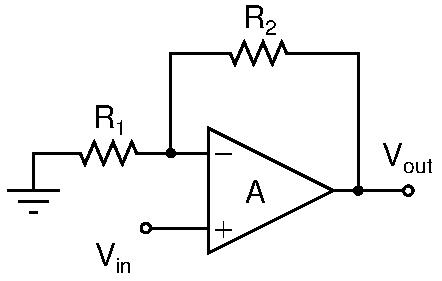
\includegraphics[height=1in]{./schematics/noninv_ampl}\\
	\begin{parts}
		\part[10]
		Find the expression for the output voltage in terms of $V_{in}$,
		$R_1$, $R_2$, and $A$. Do not assume that $A$ is infinite.
		\vskip 2.5in
		$V_{out}=$
		\part
		If the gain bandwidth product $A(f) \times f = 10$~MHz.
		$R_2/R_1=10$.
		\begin{subparts}
			\subpart[5]
			What is the gain of the system at 10~Hz
			\vskip 0.5in
			$G(10~Hz)=$
			\subpart[5]
			What is the gain of the system at 10~MHz
			\vskip 0.5in
			$G(10~MHz)=$
		\end{subparts}

		\part[5]
		Consider the practical limitations now.
		If  $R_2/R_1=99$, $V_{in}=0.01$~V, and $A=\infty$, 
		but maximum output current of the
		Op-amp is 2~mA. What is the minimal possible load resistor which you
		can hook to the output without overloading the Op-amp?
		Assume that $R_2 \gg R_L$.

		\vskip 0.5in
		$R_{L_{min}}=$
		\bonuspart[5]
		What is the output impedance of this amplifier at low
		frequencies?  
		{\bf Why} do you think so?
		Assume $A=\infty$.
		\vskip 0.4in
		$Z_{out}=$
	\end{parts}
	\pagebreak


	% -*- latex -*-
% FILE: "/home/evmik/jobs/wm/2012_spring_Analog_Electronics_252/final_exam/questions/math_with_opamps.tex"
% LAST MODIFICATION: "Tue, 01 May 2012 01:11:51 -0400 (evmik)"
% (C) 2011 by Eugeniy Mikhailov, <evgmik@gmail.com>
% $Id:$

\question{}
	\begin{parts}
		\part[20]
		Design (use as many Op-Amps as needed)
		and sketch a circuit which output is governed by the following
		expression. 
		\begin{equation}
			V_{out}=-5(V_1+ V_2) + 10 V_3
		\end{equation}
		Explain your design.
		Specify all relevant components values, assume that you are using
		ideal Op-Amps (open loop gain $A=\infty$).

		\bonuspart[5]
		{\bf Note:} You will get it if you use only one Op-Amp.

		\vskip 2.5in
	\end{parts}
	\pagebreak


	% -*- latex -*-
% FILE: "/home/evmik/jobs/wm/2012_spring_Analog_Electronics_252/final_exam/questions/oscillator.tex"
% LAST MODIFICATION: "Tue, 01 May 2012 14:21:05 -0400 (evmik)"
% (C) 2011 by Eugeniy Mikhailov, <evgmik@gmail.com>
% $Id:$

\question{}
	Consider the relaxation oscillator base on the open collector
	comparator shown below with the following parameters:\\
	$R_1=100$~k$\Omega$, $R_2=100$~k$\Omega$, $R_f=100$~k$\Omega$, and
	$R_{{p.up}}$=1~k$\Omega$.
	\begin{parts}
		\part[2]
		Disregarding $R_{{p.up}}$.
		What is the voltage at non-inverting input when output is
		high?
		\\
		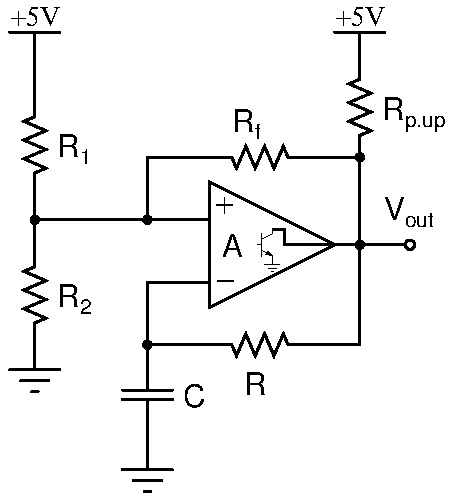
\includegraphics[height=2in]{./schematics/oscillator}
		$V_{+}=$
		\part[2]
		Disregarding $R_{{p.up}}$.
		What is the voltage at non-inverting input when output is
		low?
		\vskip 1.0in
		$V_{+}=$
		\part[4]
		If $R=1$~M$\Omega$, what is the value of the capacitor to
		get period of oscillation T=$1$~mS?
		\vskip 1.0in
		$C=$
		\part[2]
		Can we completely get rid of $R_{p.up}$? Why?
		\vskip 1.0in
		\bonuspart[5]
		When we built a blinker, we learn that hooking an LED
		directly to the output is bad idea die to large output
		impedance in comparison to the small input impedance of the
		LED. What is the output impedance of this circuit? {\bf
		Show} your reasons.
		\vskip 1.0in
		$Z_{out}=$
	\end{parts}
	\pagebreak


	% -*- latex -*-
% FILE: "/home/evmik/jobs/wm/2011_spring_Analog_Electronics_252/final_exam/questions/output_impedance_of_fancy_opamp_amplifiers.tex"
% LAST MODIFICATION: "Thu, 05 May 2011 12:14:47 -0400 (evmik)"
% (C) 2011 by Eugeniy Mikhailov, <evgmik@gmail.com>
% $Id:$

\question{}
In this problem assume that you have an ideal Op-amp (the open loop gain $A=\infty$).
	\begin{parts}
		\part
		Consider the circuit below \\
		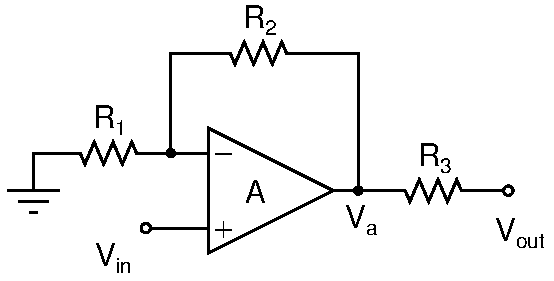
\includegraphics[height=1in]{./schematics/noninv_ampl_with_output_resistor}\\
		\begin{subparts}
			\subpart[5]
			Express $V_a$ and $V_{out}$ as function of $V_{in}$ and circuit
			components assuming no load connected.
			\vskip .8in
			\subpart[5]
			Assume that dummy load with resistance $R_L$ is
			connected to the output. Which of the voltages
			$V_a$ or $V_{out}$ depend on $R_L$?
			\vskip .8in
			\subpart[5]
			Using above find the output impedance of this
			circuit.
			\vskip .8in
		\end{subparts}

		\part
		Consider the circuit below \\
		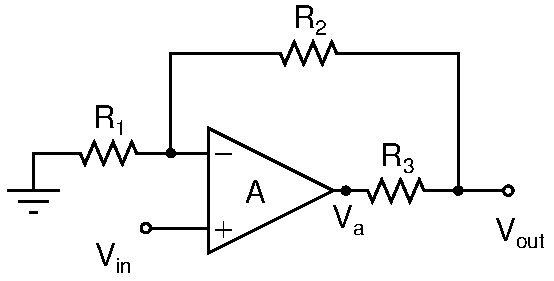
\includegraphics[height=1in]{./schematics/noninv_ampl_with_output_resistor_in_feedback}\\
		\begin{subparts}
			\subpart[5]
			Express $V_a$ and $V_{out}$ as function of $V_{in}$ and circuit
			components assuming no load connected.
			\vskip .8in
			\subpart[5]
			Assume that dummy load with resistance $R_L$ is
			connected to the output. Which of the voltages
			$V_a$ or $V_{out}$ depend on $R_L$? Hint: it is
			easier to find $V_{out}$ if you consider the
			current through $R_2$ and $R_1$.
			\vskip .8in
			\subpart[5]
			Using above find the output impedance of this
			circuit.
			\vskip .8in
		\end{subparts}
	\end{parts}

	\pagebreak

	% -*- latex -*-
% FILE: "/home/evmik/jobs/wm/2011_spring_Analog_Electronics_252/final_exam/questions/matched_njfet_follower.tex"
% LAST MODIFICATION: "Thu, 05 May 2011 10:50:43 -0400 (evmik)"
% (C) 2011 by Eugeniy Mikhailov, <evgmik@gmail.com>
% $Id:$

\question{}
	Consider the circuit shown below. \\
	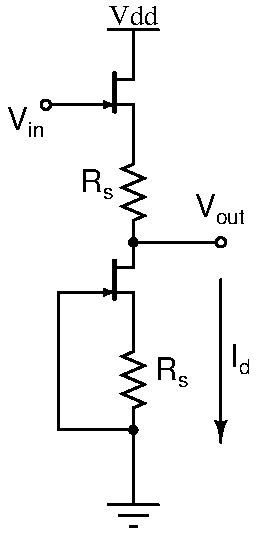
\includegraphics[height=2in]{./schematics/njfet_matched_follower}\\
	NJFETs in this circuit are {\bf  matched}. 
	Presume that $V_{dd}$ is large enough for transistors to be in saturation.
	\begin{parts}
		\part[5]
		First consider only bottom part (below $V_{out}$ terminal). It can be
		thought as a constant current source with current $I_d$ (assume that it
		is somehow known to you).
		
		Write the {\bf symbolical} expression for the $V_{GS}$ of the bottom transistor.
		\vskip .5in
		$V_{GS}=$

		\part[15]
		Using above information. Derive the {\bf symbolical} expression for the output
		voltage  $V_{out}$ in terms of the input voltage, $V_{GS}$, $I_d$,  and
		$R_s$. {\bf Hint:} you might not need all of them at the very end. 
		\vskip 1.8in
		$V_{out}=$

		\part
		The  transistors parameters are the following: the pinch off voltage
		$V_p=-2$~V, the coefficient $k=2\times10^{-3}$~A/(V$^2$). Supply
		voltage $V_{dd}=20$~V, $R_s=500$~$\Omega$. 
		\begin{subparts}
			\subpart[5]
			Find  the quiescent current supplied by the power supply.
			\vskip 1in
			$I_{d}=$

			\subpart[5]
			Find  the quiescent power dissipated by this circuit
			\vskip .5in
			$P_{q}=$
		\end{subparts}

	\end{parts}
	\pagebreak



\end{questions}
\end{document}

% vim: tabstop=2 shiftwidth=2 

